\section{Características del Robot} \label{sec:caracteristicas_del_robot}

El robot utilizado en este proyecto es un manipulador articulado de varios grados de libertad, cuya estructura fue previamente dise\~nada en SolidWorks. Este tipo de robot est\'a compuesto por una serie de eslabones y articulaciones conectadas en serie, lo que le permite alcanzar una variedad de posiciones y orientaciones en el espacio tridimensional.

\begin{figure}[H]
	\centering
	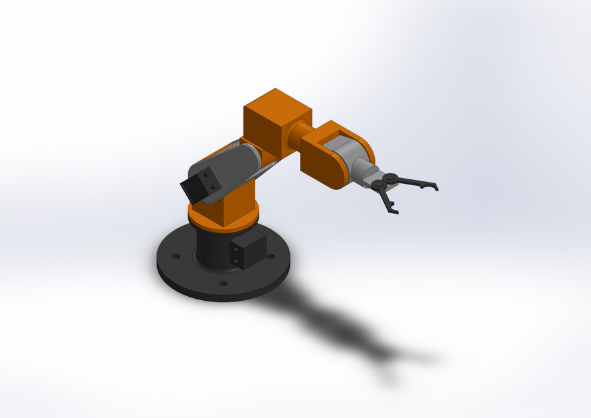
\includegraphics[width=0.7\textwidth]{caracteristicas del robot}
	\caption{Características del robot utilizado en el proyecto.}
	\label{fig:caracteristicas_robot}
\end{figure}


	La tabla de Denavit-Hartenberg (DH) es una herramienta fundamental para describir la geometría cinemática de un robot manipulador. Esta tabla resume los parámetros geométricos necesarios para modelar la posición y orientación relativa entre los eslabones adyacentes del robot.
\begin{table}[ht]

	\centering
	\caption{Parámetros de Denavit Hartenberg y límites del robot}
	\label{tab:parametros_robot}
	\begin{tabular}{ l|cccccccccccc
		}
		\toprule
		N & {$\theta$} & {$d$} & {$a$} & {$\alpha$} & {tipo} 
		& {$q_{\min}$} & {$q_{\max}$} 
		& {$\dot q_{\max}$} & {$\ddot q_{\max}$} 
		& {$\tau$} & {$\mu_s$} & {$\mu_k$} \\
		\midrule
		1 & 0 & 95 & 0  & -90   & r & -90 & 90 & 180 & 360 &  1.041  & 0.1 & 0.2 \\
		2 & -90 & 0 & 152  & 0 & r & -90 & 180 & 180 & 360 & 2.31  & 0.1 & 0.2 \\
		3 & 90 & 0 & 167  & 0 & r & -90 & 180 & 180 & 360 & 2  & 0.1 & 0.2 \\
		4 & -90 & 80 & 0  & -90   & r &   -90 &  180 &   180 &   360 & 0.6  & 0.1 & 0.2 \\
		\bottomrule
	\end{tabular}
\end{table}
\bigskip
\noindent
\begin{description}
	\item[N] Número de la articulación.
	\item[\(\theta\)] Ángulo articular (grados).
	\item[\(d\)] Desplazamiento articular (mm).
	\item[\(a\)] Longitud del eslabón (mm).
	\item[\(\alpha\)] Ángulo de torsión DH (grados).
	\item[tipo] ‘r’ para articulación rotacional, ‘p’ para prismática.
	\item[\(q_{\min}\), \(q_{\max}\)] Límites de posición (grados o mm).
	\item[\(\dot q_{\max}\)] Límite de velocidad (grados/s o m/s).
	\item[\(\ddot q_{\max}\)] Límite de aceleración (grados/s² o m/s²).
	\item[\(\tau\)] Torque o fuerza máxima permitido (\(N \cdot m\) o \(N\)).
	\item[\(\mu_s\)] Fricción estática (\(N\) o \(N \cdot m\)).
	\item[\(\mu_k\)] Fricción cinética (\(N \cdot m \cdot s\) o \(\frac{N \cdot m \cdot s}{rad}\)).
\end{description}

